%%%%%%%%%%%%%%%%%%%%% chapter.tex %%%%%%%%%%%%%%%%%%%%%%%%%%%%%%%%%
%
% sample chapter
%
% Use this file as a template for your own input.
%
%%%%%%%%%%%%%%%%%%%%%%%% Springer-Verlag %%%%%%%%%%%%%%%%%%%%%%%%%%

\chapter{Nonparametric Techniques}\label{metodinonparametrici}

\section{introduzione}
Nella sezione \ref{tecnicheParametriche} sono state trattate  le tecniche parametriche nel caso di addestramento \emph{supervised} assumendo una distribuzione di probabilità nota. Purtroppo nelle applicazioni di \emph{pattern recognition} non sempre abbiamo una conoscenza della distribuzione di probablità. In questa sezione verranno esaminate quelle tecniche chiamate \emph{nonparametric} che possono essere usate arbitrariamente con qualsiasi distribuzione senza assumere una conoscenza a priori. Ci sono molte tipologie di tecniche \emph{nonparametric}: in particolare una consiste nella procedura di stimare la funzione di densità $p(\mathbf{x}|\omega_j)$ dai campioni di \emph{patterns}, mentre un altra tecnica consiste invece in una procedura che stima direttamente la la probablità a posteriori $P(\omega_j|\mathbf{x})$.

\section{Stima della densità}
La probabilità $P$ che un vettore $\mathbf{x}$ ricade in una regione di decisione $\mathcal{R}$ è data da
\begin{equation}\label{P}
P = \int_{\mathcal{R}} p(\mathbf{x}') \ d\mathbf{x}'
\end{equation}
stiamo calcolando l'area che sottende la probabilità del campione $\mathbf{x}'$ all'interno della regione di decisione. $P$ è la versione media della funzione di densità $p(\mathbf{x})$, e possiamo stimare il valore di $p$ calcolando la probabilità $P$. Supponiamo di avere $n$ campioni $\mathbf{x}_1, \dots, \mathbf{x}_n$  che sono indipendenti e identicamente distribuiti (\emph{i.i.d.}) secondo la funzione di probabilità non nota $p(\mathbf{x})$. La probabilità che $k$ di questi $n$ campioni cada nella regione di decisione $\mathcal{R}$ è data dal coefficiente binomiale, ovvero la probabilità che $k$ degli $n$ campioni ricadano all'interno di una regione di decisione
\begin{equation}
P_k = \binom{n}{k} P^k (1-P)^{n-k}
\end{equation}
dove $P^k$ è la probabilità dei $k$ campioni che ricadono all'interno della regione $\mathcal{R}$, $(1-P)^{n-k}$ è la probabilità che $k$ campioni non ricadono all'interno della regione $\mathcal{R}$ e $\binom{n}{k}$ è il coefficiente binomiale, moltiplicando il tutto otteniamo $P_k$ che prende il nome di distribuzione binomiale. Inoltre il valore atteso di $k$ è
\begin{equation}
\varepsilon[k] = nP
\end{equation}
a questo punto vogliamo trovare quel parametro $k$ tale che abbiamo proprio la probabilità media, quindi se cambio il numero di campioni questa regola permane. Qual'è il valore per il quale ottengo esattamente $nP$? \'E proprio $k$. Con questa supposizione $k$ è approssimatiamente uguale ad $nP$, quindi essendo $k \simeq nP$, allora $P \simeq k/n$ sostituisco nella \ref{P} e di conseguenza otteniamo
\begin{equation}
\frac{k}{n} \simeq \int_{\mathcal{R}} p(\mathbf{x}') \ d\mathbf{x}'
\end{equation}
Individuata la regione di appartenenza dei punti, ipotizziamo di sceglierla piccola in modo tale da avere una densità della probabilità costante all'interno di essa, a questo punto la $p(\mathbf{x}')$ risulta essere costante rispetto ad $\mathbf{x}'$ e quindi è possibile portarla al di fuori dell'integrale e quindi il tutto diventa
\begin{equation}
\frac{k}{n} \simeq p(\mathbf{x}) \int_{\mathcal{R}} d\mathbf{x}'
\end{equation}
L'integrale $ \int_{\mathcal{R}} d\mathbf{x}'$ non è altro che un volume, quindi ho $p(\mathbf{x})V$, riprendendo la formula precedente 
\begin{equation}
\frac{k}{n} \simeq p(\mathbf{x})V
\end{equation}
riarrangiando viene fuori che una stima di $p(\mathbf{x})$ potrebbe essere
\begin{equation}\label{densita}
p(\mathbf{x}) = \frac{k/n}{V}
\end{equation}
dove $k$ è il numero di campioni che rientrano nella regione $\mathcal{R}$, $n$ è il numero di campioni in totale e $V$ è il volume della regione $\mathcal{R}$. Ci troviamo di fronte ad un equazione di cui $p(\mathbf{x})$, $k$ e $V$ non sono noti e conosciamo solo $n$. Quindi è necessario introdurre altre considerazioni. Per vedere il comportamento di $n$ tendente ad infinito della (\ref{densita}) allora consideriamo $n$ molto grande , per fare questo scriviamo 
\begin{equation}\label{densita1}
p_n(\mathbf{x}) = \frac{k_n/n}{V_n}
\end{equation}
quindi otteniamo la stima della densità di probabilità di $\mathbf{x}$ al variare di $n$, osservando che più $n$ cresce più la \ref{densita1} tenda alla vera densità di probabilità. Andiamo a calcolare il limite tendente all'infinito delle quantità che entrano in gioco. C'è da considerare che il limite per $n$ tendente all'infinito della \ref{densita1} è una forma indeterminata $0/\infty$, quindi va studiata singolarmente, in particolare pretendiamo che il volume non cresca all'infinito. Se $p_n(\mathbf{x})$ deve convergere a $p(\mathbf{x})$ allora sono rischieste tre condizioni: 
\begin{itemize}
\item $\lim_{n\to \infty} V_n = 0$
\item $\lim_{n\to \infty} k_n = \infty$
\item $\lim_{n\to \infty} k_n/n = 0$
\end{itemize}
La prima condizione assicura che il volume non cresca all'infinito, quindi aumentando i campioni la regione rimane constante, al più si rimpicciolisce ma non aumenta. La seconda condizione, la quale ha senso soltanto se $p(\mathbf{x}) \neq 0$ ci assicura che il rapporto convergerà alla probabilità $P$. Ci sono due modi per soddisfare le condizioni (Fig. \ref{px}). Uno è quello di considerare una regione iniziale $V_n$ in funzione di $n$, come $V_n = 1/\sqrt{n}$, inquesto caso deve essere dimostrato che le variabili casuali $k_n$ e $k_n / n$ si comportano correttamente o, più precisamente, che $p_n(\mathbf{x})$ converge a $p(\mathbf{x})$, questo è il metodo \emph{parzen windows} che verrà esaminato a breve. Il secondo metodo invece considera $k_n$ in funzione di $n$, esempio $k_n = \sqrt{n}$, in questo caso il volume è cresciuto fino a racchiudere $k_n$ vicini di $\mathbf{x}$, questa tecnica è chiamata stima \emph{$k_n$-nearest-neighbor}.

\begin{figure}
\centering
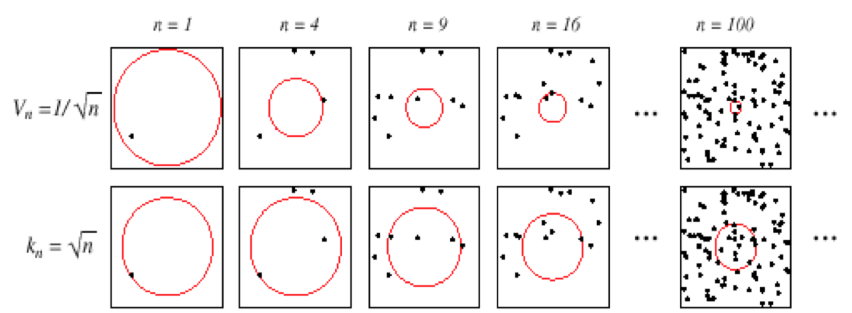
\includegraphics[scale=0.5]{img/px.png}
\caption{Metodi per la stima di densità di probabilità}
\label{px}
\end{figure}

\section{Parzen Windows}
L'approccio denominato \emph{Parzen Windows} può essere introdotto assumendo che la regione $\mathcal{R}_n$ è un ipercubo a $d$ dimensioni. Se $h_n$ è la lunghezza del lato dell'ipercubo allora il suo volume è dato da
\begin{equation}
V_n = h_n^d
\end{equation}
A questo punto viene introdotta la funzione finestra, la quale dice: se un campione rientra in un cubo assume valore 1 altrimenti assume valore 0.  
\[
\varphi(\mathbf{u})=
\begin{cases}
1 & \text{se} \ \abs{u_j} \leq 1/2\\
0 & \text{altrimenti}
\end{cases} 
\quad \quad \quad
j = 1, \dots, d.
\]
Facciamo un esempio a due dimensioni ed immaginiamo un quadrato centrato nell'origine, allora il valore delle due dimensioni deve essere $\abs{u_j} \leq 1/2$ per poter rientrare all'interno del quadrato, altrimenti si trova al di fuori. In questo caso è stato assunto che il lato abbia dimensione unitaria e che l'ipercubo sia centrato nell'origine. Volendo applicarla al caso generale è necessario traslare nell'origine e poi dividere per $h_n$, quindi la funzione finestra divente $\varphi((\mathbf{x} - \mathbf{x}_i)/h_n)$. Una volta ottenuta la funzione finestra per il caso generale la applico a tutti i punti per vedere quanti campioni rientrano all'interno della regione. Il che può essere calcolato con la sommatoria per tutti gli $i=1$
\begin{equation}
k_n = \sum_{i=1}^n \varphi \left ( \frac{\mathbf{x} - \mathbf{x}_i}{h_n} \right )
\end{equation}
così $k_n$ lo calcolo e non si fa nessuna ipotesi, mentre si fa l'ipotesi sul volume che come abbiamo detto è uguale a $h_n^d$. Sostituiamo $k_n$ nella formula originaria
\begin{equation}
p_n(\mathbf{x}) = \frac{k_n/n}{V_n}
\end{equation}
e ottengo
\begin{equation}\label{stima}
p_n(\mathbf{x}) = \frac{1}{n} \sum_{i=1}^n \frac{1}{V_n}\varphi \left ( \frac{\mathbf{x} - \mathbf{x}_i}{h_n} \right )
\end{equation}
La stima appena vista è basata sul concetto del conteggio del numero di campioni di training contenuti in un volume prefissato, quindi la stima della distribuzione di probabilità è espressa come somma di $N$ contributi, ciascuno dei quali è associato ad un singolo campione, ed il singolo contributo è espresso da una funzione $\varphi(\mathbf{u})$ che in generale non è rettangolare ($\varphi(\mathbf{u})$ ma assume valori continui. Si costruisce quindi la stima mediante l'equazione \ref{stima}. La funzione  $\varphi(\mathbf{u})$ è detta finestra di Parzen o \emph{kernel}.\\

\noindent Affinchè lo stimatore di Parzen abbia significato, è necessario imporre vincoli sul kernel $\varphi(\mathbf{u})$. Una condizione necessaria e sufficiente affinchè la stima di Parzen sia effettivamente una distribuzione di probabilità, è che la stessa funzione \emph{kernel} sia una distribuzione di probablità, ossia una funzione non-negativa
\begin{equation}
\varphi(\mathbf{x}) \geq 0
\end{equation}
e normalizzata
\begin{equation}
\int \varphi(\mathbf{u}) \ d\mathbf{u} = 1
\end{equation}
Definiata la funzione $\delta_n(\mathbf{x})$
\begin{equation}
\delta_n(\mathbf{x}) = \frac{1}{V_n} \varphi \left ( \frac{\mathbf{x}}{h_n} \right )
\end{equation}
allora la distribuzione di probabilità può essere scritta anche in un altra forma
\begin{equation}
p(\mathbf{x}) = \frac{1}{n} \sum_{i=1}^n \delta_n(\mathbf{x} - \mathbf{x}_i)
\end{equation}
Osserviamo come cambia la finestra di parzen al variare di $k_n$. I vari casi sono mostrati in figura \ref{parzen}.
\begin{figure}
\centering
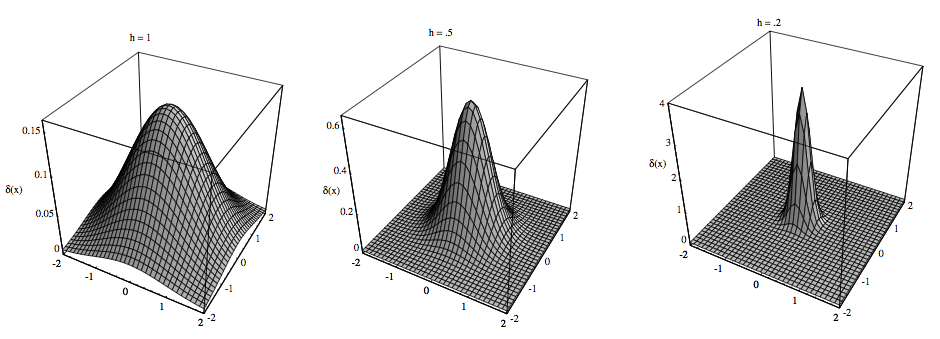
\includegraphics[scale=0.4]{img/parzen.png}
\caption{Finestre di parzen con $k_n$ variabile}
\label{parzen}
\end{figure}
Diminuendo $h_n$ il volume diventa più piccolo e di conseguenza $\delta_n$ ha un picco maggiore, di volta in volta che $h_n$ diminuisce il picco aumenta, quindi per $h_n$ tendente a zero diventa proprio la delta di dirac. Se invece $h_n$ è grande allora assume la forma di una gaussiana con varianza molto ampia ma con lo svantaggio che è poco rappresentativa dei pattern, quindi potrebbe essere che la distribuzione di probabiità non è costante di conseguenza stiamo perdendo molte informazioni dei pattern all'interno di questa regione (Regione grade equvale a perdita di informazioni). Analogamente invece $h_n$ è troppo piccolo allora guardiamo molti dettagli e nel tendere alla delta di dirac è come se stessimo osservando un singolo campione. Ritornando alla discussione sulla convergenza, bisogna tener conto della convergenza della sequenza delle variabili casuali, dato che per ogni fissato $\mathbf{x}$ il valore di $p(\mathbf{x})$ dipende dai campioni $\mathbf{x}_1, \dots, \mathbf{x}_n$. Quindi se la media di $p_n(\mathbf{x})$ è $\bar{p}_n(\mathbf{x})$ e la varianza è $\sigma^2_n(\mathbf{x})$. Allora la stima di $p_n(\mathbf{x})$ converce a $p(\mathbf{x})$ se
\begin{equation}
\lim_{n \to \infty} \bar{p}_n(\mathbf{x}) = p(\mathbf{x})
\end{equation}
e
\begin{equation}
\lim_{n \to \infty} \sigma^2_n(\mathbf{x}) = 0
\end{equation}

\subsection{Esempi}
\'E interessante vedere come  si comporta il metodo \emph{parzen windows} ed in particolare osservare l'effetto della funzione finestra. Consideriamo il caso in cui $p(\mathbf{x})$ è una distribuzione normale monovariata a media zero e varianza unitaria. L funzione finestra avrà la seguente forma
\begin{equation}
\varphi(u) = \frac{1}{\sqrt{2\pi}} e^{-u^2/2}
\end{equation}
dato $h_n = h_1/\sqrt{n}$. Allora $p_n(x)$ è una distribuzione di densità centrata sui campioni
\begin{equation}
p_n(x) = \frac{1}{n} \sum_{i=1}^n \frac{1}{h_n} \varphi \left ( \frac{x - x_i}{h_n} \right)
\end{equation}
\begin{figure}
\centering
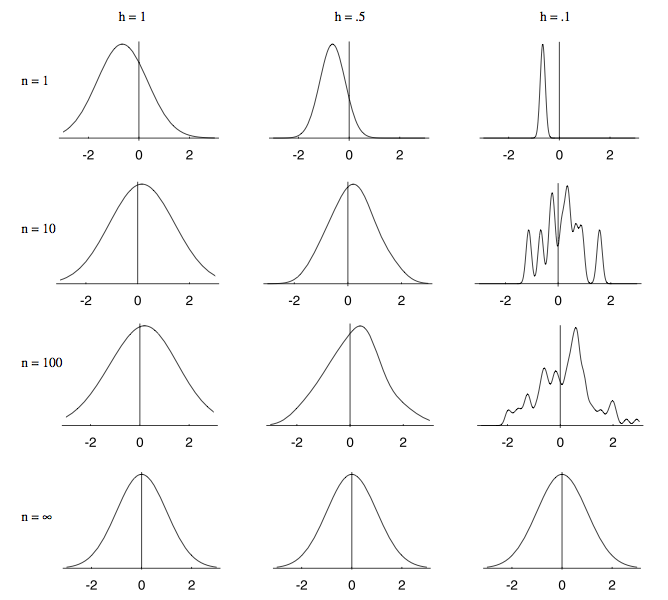
\includegraphics[scale=0.5]{img/parzen1.png}
\caption{Stima mediante la tecnica \emph{Parzen window} di una distribuzione normale monovariata facendo variare il parametro $h_1$ ed il numero di campioni $n$}
\label{parzen1}
\end{figure}
Effettuando un pò di calcoli sono stati ottenuti i risultati mostrati in figura \ref{parzen1}. I risultati dipendono sia da $h_1$ che da $n$. Per $n=1$ e $h_1=1$ è semplicemente una gaussiana centrata sul primo campione, quindi una visione sfocata \emph{out-of-focus} della distribuzione. Per $n=10$ e $h_1 = 0.1$ osserviamo che si può distinguere il contributo di ogni campione cosa che non avviene nel caso in cui $h_1=1$ e $h_1=0.5$. 

\subsection{Classificazione}
Una volta stimata la densità di probabilità allora la classificazione viene effettuata mediante una stima a massima probabilità a posteriori (MAP). Le regioni di decisioni dipendono dalla scelta che si fa per la funzione finestra. In generale, l'errore è basso scegliendo finestre con dimensione piccola.

\section{$k_n$-Nearest Neighbor estimation}
 Un rimedio al problema della dimensione della finestra di parzen è quello di considerare il volume in funzione dei campioni di training. Per esempio, per stimare la $p(\mathbf{x})$ di un insieme di campioni di training, possiamo centrare la regione in $\mathbf{x}$ e farla crescere finchè ingloba $k_n$ campioni, dove $k_n$ è specificato in funzione di $n$. Questi campioni sono i $k_n$ \emph{nearest-neighbor} di $\mathbf{x}$. Se vicino il campione $\mathbf{x}$ la densità è alta allora la cella sarà piccola, viceversa se la densità è bassa allora si avrà una regione grande. In entrambi i casi se prendiamo
 \begin{equation}\label{stima1}
p_n(\mathbf{x}) = \frac{k_n/n}{V_n}
\end{equation}
vogliamo che sia $k_n$ ed $n$ tendono ad infinito dato che ci assicura che $k_n/n$ sarà una buona stima di probabilità che un punto cadrà all'interno del volume $V_n$. Comunque, vogliamo anche che $k_n$ cresce lentamente finchè la dimensione della cella non include i $k_n$ campioni. \'E chiaro che dalla \ref{stima1} il rapporto $k_n/n$ tende a zero. Si può dimostrare che le condizioni $\lim_{n \to \infty} k_n = \infty$ e $\lim_{n \to \infty} k_n/n = 0$ sono necessarie e sufficienti affinchè $p_n(\mathbf{x})$ converge a $p(\mathbf{x})$. Se poniamo $k_n=\sqrt{n}$ e assumiamo che $p_n(\mathbf{x})$ è una buona approssimazione di $p(\mathbf{x})$ allora dall'eq. \ref{stima1} otteniamo che $V_n \simeq \/(\sqrt{n} \ p(\mathbf{x}))$. Così $V_n$ ha ancora la forma $V_1/\sqrt{n}$, ma il volume iniziale è determinato dalla natura dei dati piuttosto che da una scelta arbitraria. \'E interessante notare che nonostante $p_n(\mathbf{x})$ è continua la sua pendenza (o gradiente) non lo è. Inoltre i punti di dscontinuità corrispondono ai punti stessi (Fig. \ref{knn1} e \ref{knn2}).

\begin{figure}
\centering
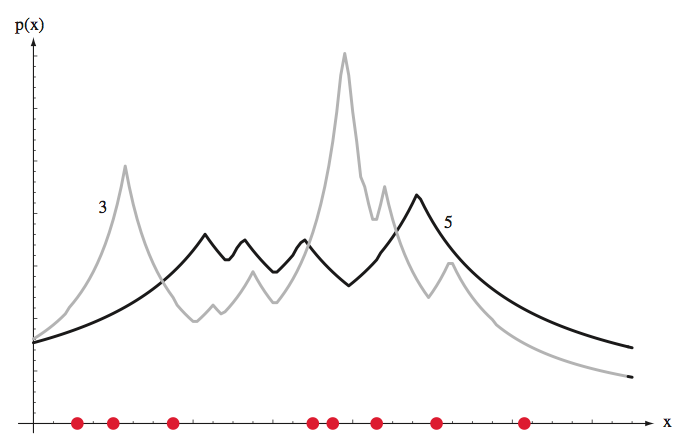
\includegraphics[scale=0.33]{img/knn1.png}
\caption{}
\label{knn1}
\end{figure}

\begin{figure}
\centering
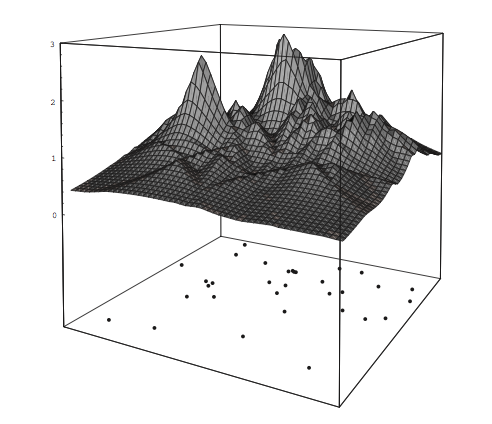
\includegraphics[scale=0.5]{img/knn2.png}
\caption{}
\label{knn2}
\end{figure}

\subsection{$K_n$-Nearest-Neighbor and Parzen Window Estimation }
Nel caso in cui $n=1$ allora $k_n = \sqrt{n} = 1$ e quindi i questo caso la stima diventa
\begin{equation}
p_n(x) = \frac{1}{2\abs{x-x_1}}
\end{equation}
\'E il caso in cui il numero di campioni più prossimi ad $x$ sia $1$, portando ad una tecnica denominata \emph{one-nearest-neighbor}

\subsection{Estimation of \emph{A Posteriori} Probabilities}
Le tecniche discusse nelle precedenti sezioni possono essere usate per stimare la probabilità a posteriori $P(\omega_i|\mathbf{x})$ da un insieme di $n$ campioni etichettati usando gli stessi campioni per stimare le densità coinvolte. Supponiamo di utilizzare una volume $V$ intorno ad $\mathbf{x}$ e catturare i $k$ campioni, $k_i$ di questi sono etichettati con $\omega_i$. La stima della probabilità congiunta $p(\mathbf{x} \cap \omega_i)$ è 
\begin{equation}
p_n(\mathbf{x} \cap \omega_i) = \frac{k_i/n}{V}
\end{equation}
quindi la stima di $P(\omega_i | \mathbf{x})$ è
\begin{equation}
P_n(\omega_i | \mathbf{x}) = \frac{p_n(\mathbf{x} \cap \omega_i)}{\sum_{j=1}^c p_n(\mathbf{x} \cap \omega_j)} = \frac{k_i}{k}
\end{equation}
La probabilià a posteriori che il campione appartenga alla classe $\omega_i$ è data dal rapporto tra il numero campioni etichettati con $\omega_i$ ed i campioni $k$ all'interno del volume. Per la scelta della grandezza della cella è chiaro che possiamo usare sia l'approccio basato sulle finestre di parzen che quello basato sul $k_n$\emph{-nearest-neighbor}. Nel primo caso $V_n$ deve essere specificato come funzione di $n$, come $V_n = 1/\sqrt{n}$. Nel secondo caso, $V_n$ viene esteso fino a racchiudere un determinato numero di campioni, es. $k = \sqrt{n}$. 

\subsection{The Nearest-neighbor rule}
Sia $\mathcal{D}^n = \{\mathbf{x}_1, \dots, \mathbf{x}_n \}$ un insieme di $n$ campioni dei quali conosciamo la classe di appartenenza (approccio supervisionato), preso $\mathbf{x}' \in \mathcal{D}^n$ come più vicino prossimo al campione $\mathbf{x}$ che è un campione di test (quindi non appartiene al dataset). La regola nearest-neighbor assegna ad $\mathbf{x}$ l'etichetta di $\mathbf{x}'$. Il tasso di errore è certamente maggiore di quello della regola di bayes, cioè quella del minimo possibile, però si dimostra che il tasso di errore è al più due volte l'errore di bayes, cioè è limitato superiormente da due volte l'errore di bayes. L'errore di bayes è molto piccolo, quindi moltiplicato per due è ancora piccolo. Questo è il vantaggio che può dare il nearest-neighbor con $k=1$, quindi costo computazionale bassissimo con grossa resa, dato che per $n$ tendende ad infinito la probabilità di $p(\omega_i|\mathbf{x}') \simeq p(\omega_i|\mathbf{x})$, cioè i vicini hanno probabilità a posteriori costanti. Inoltre se $p(\omega_m|\mathbf{x}') \simeq 1$, qundi molto alta, allora in tal caso il comportamento del classificatore nearest-neighbor è uguale al comportamento di bayes. 
\begin{figure}
\centering
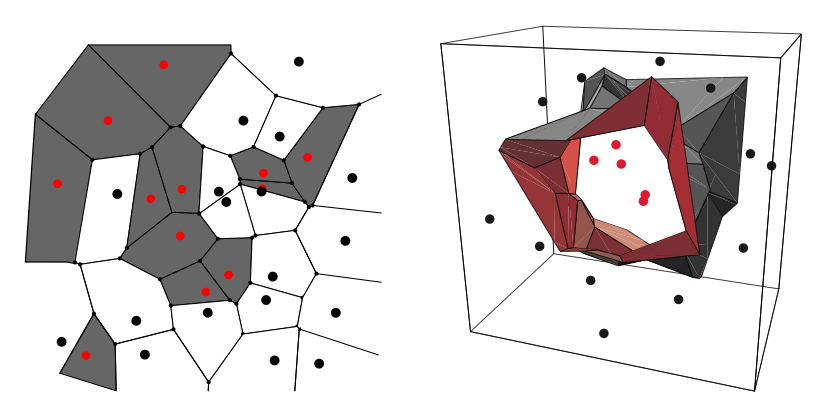
\includegraphics[scale=0.4]{img/voronoi.png}
\caption{Tassellazione di voronoi, le frontiere di decisione sono come superfici di diamanti}
\label{voronoi}
\end{figure}
Stiamo dicendo che una regola di classificazione banale ha un comportamento molto valido. Generalizzando, il \emph{k-nearest-neighbord} assegna ad $\mathbf{x}$ l'etichetta del campione più frequentemente rappresentato dei $k$ campioni più vicini. L'algoritmo conduce quindi ad un partizionamento, una cosa interessante in quanto ho delle celle intorno ad ogni campione $\mathbf{x}$. La suddivisione delle celle viene definita tassellazione di voronoi, fondamentalmente è un partizionamento senza sovrapposizione delle celle (Fig. \ref{voronoi}). \\

\noindent Nota: Se aumento il numero di $k$ vicini le regioni sono dense e i picchi si abbassano, invece se $k$ diminuisce allora ci sono più picchi.


%
